\documentclass{article}
\usepackage[utf8]{inputenc}
\usepackage{graphicx}
\usepackage{amsmath}
\usepackage{subfig}
\usepackage{titlesec}
\usepackage{hyperref}
\graphicspath{ {./images/} }
\usepackage{float}
\usepackage[margin=1in]{geometry}
\hypersetup{
    colorlinks=true,
    linkcolor=blue,
    filecolor=magenta,
    urlcolor=cyan,
    pdftitle={Overleaf Example},
    pdfpagemode=FullScreen,
    }

\title{Code Theory Project\\\\ University Antwerp}
\author{Cédric Leclercq, Elias Dams, Robbe Nooyens}
\date{December 2022}

\begin{document}

\maketitle

\tableofcontents

\newpage

\section{VigenerePlus (Elias Dams)}
\subsection{About}
VigenèrePlus is a chipher in which first Vigenère and then single column transposition is applied. Two different keywords are used in this process.\\
\\
I found it very difficult to find a suitable approach. Vigenère's weaknesses are Kasiski's test and coincidence index. However, if you put column transposition on top of Vigenère, that weakness is gone. The text is now shuffled and you can't search for digraphs/trigraphs because they give the wrong key length pattern. Nor can you solve for Columnar Transposition because the resulting text is still encrypted with Vigenère.\\
\\
If we want to brute force (assuming we both have keys with a maximum length of 10). we have to go through all the permutations. This not possible, as makes a total of 16304741395569 possibilities: \\
\\
$\sum_{i=1}^{10} i! \cdot \sum_{j=1}^{10} j! = 16304741395569$\\

\subsection{Single-column transposition}
We must first solve the column transposition. We do this by going over all possible permutations of maximum length 10 (otherwise it takes a long time) and making a selection. So we will have to identify how hard a transposed cypher text resembles a Vigenère chipher. As mentioned earlier, a coincidence index will not say much because only the order of the letters changes.\\
\\
What we can do however is run a Kasiski test. Kasiski suggested looking for repeated fragments in the cipher text and making a list of the distances separating the repetitions. Then the length of the keyword is likely to divide many of these distances. With a non Vigenère text this test will not be of much use and all key lengths are equally possible. However, with a Vigenère text there will often be an outlier of a possible key length. If there is such an outlier it gets written to a file. After a run of the first part of my algorithm we have a file consisting of all the Vigenère cipher texts with a possible Vigenère key length. So we have reduced the number of possibilities considerably. If the outlier had a length smaller than 4, I manually remove it, because this would be an unrealistically small key.\\

\subsection{Vigenère}
Now we only have a list of vigenere encrypted messages and their possible key lenght(s). To guess the key we are going to use the \href{http://practicalcryptography.com/media/cryptanalysis/files/english_bigrams_1.txt}{bigrams}, and their appearance in the english language. I will explain the algorithm using an example.\\
\\
Plaintext: Codetheorieproject\\
Ciphertext: Msboxfospsinbshogr\\
Key: KEY\\
\\
We loop over the text and take the doubles that are 3 positions apart (keylenght). The doubles we are going to use to determine the first letter of the key are Ms, ox, os, si, bs and og.\\

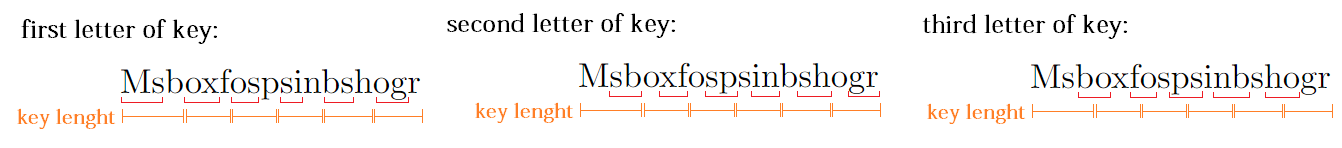
\includegraphics[scale=0.60]{image1.png}

\newpage

Then we will calculate the entropy value (from the table) of these doubles and all their possible shifts. At the end we look at the lowest entropy value. We look at the shifts. Since our key is "KEY", +11 in the example will have the lowest entropy. The 11th letter is K. This is how we determined the first letter of the key. We repeat this for each letter of the key.\\

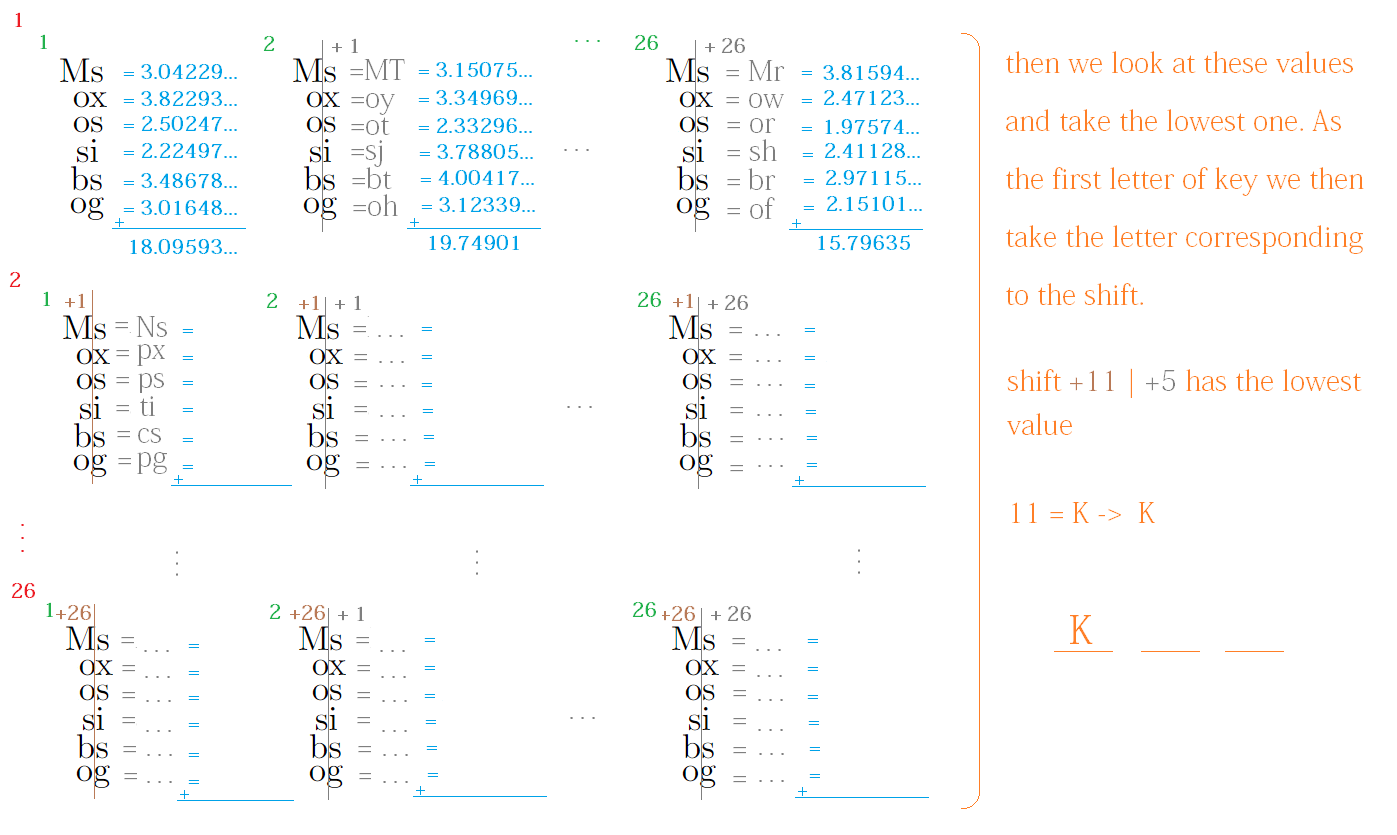
\includegraphics[scale=0.60]{image2.png}

Then we take the final key and use it to find the plaintext. Lastly, we calculate the entropy of the resulting text. If it looks like English, we write it to a file. I noticed that this doesn't always work for small texts, but the texts we got were large enough to find a correct solution each time.

\section{Playfair (Robbe Nooyens)}

\subsection{Preparation}
Before we started implementing the Playfair cracking algorithm, we first created an encode and decode algorithm. We've decided to go with a string representation of the matrix to make it easier to pass, edit and represent configurations. In order to apply the Playfair operations to the matrix to decode/encode digrams, we've made a transform function which does just this. Putting these functions together, we get the following:

\subsection{Approach 1: Bruteforce all permutations}
Our first (very naive) approach, was to generate every possible configuration. We'd then calculate how much the decoded text differed from an English text based on the mean squared error of the decoded text's letter frequencies and the letter frequencies of the English alphabet. And of course, this took ages. We've let the algorithm run until the permutation algorithm reached the letter 'p'. Since it already took an hour to reach this point, permutating all up to the letter 'a' would have taken forever. This approach would require the cracking algorithm to check 26! combinations, which is way too much. Since we also didn't know which language the text was written in, we've let it calculate the frequency score of each language, which added up to the total time.

\subsection{Approach 2: Generate keys from a dictionary}
Bruteforcing every permutation wouldn't work, so for the next attempt, we tried to narrow down the key-space. Keys or configurations for the Playfair algorithm are usually constructed as follows: Choose a word, change j's to i's, remove duplicated letters and append the rest of the alphabet. This gave me the idea to take all the words in the English alphabet and generate keys from these words. Luckily, the feedback moment took place at the right time to prevent us from spending and losing a lot of time on this ridiculous idea, since the configuration doesn't necessarily need to be an actual word.

\subsection{Approach 3: Hillclimbing with MSE}
The next approach seemed more promising. During the feedback moment, we've been given the advice to try hillclimbing or simulated annealing with the mean squared error or the vector product of the letter frequencies. We've also been told that the encrypted text was written in English, which narrowed down the checks a lot. For this new approach, we've ran this hillclimbing algorithm starting with different initial configuration for a few million times with a sufficient high depth, but this didn't yield any useful results either.

\subsection{Approach 4: Simulated annealing with MSE}
Our fourth approach was to use simulated annealing with the MSE. After doing some research, we started writing the algorithm which wasn't straightforward to do. With kMax set to 1.000.000, the results of this algorithm were already looking better, but it still didn't find the right configuration. The best scores always floated around 0.25. By using the flags -O3 and -pthread, the code could be executed relatively fast, but it still required around 16-17 minutes to complete one iteration of the algorithm. We let the algorithm run several nights, with around 20 iterations per night. Unfortunately, still none of the outcomes yielded a good result that came close to the solution.\\

\noindent As a variation on this approach, we tried combining simulated annealing with hillclimbing by making sure the algorithm could only jump to a 'worse' state if it couldn't find a better solution for some amount of consecutive iterations. Yet this didn't work either.

\subsection{Approach 5: Simulated annealing with index of coincidence}
Since we still couldn't get a decent result with recognizable words, I asked some older students which approach they suggested to try next since it still didn't work and we were out of ideas. That's how we got to know about the IC, short for 'index of coincidence'. I changed the energy function of the simulated annealing to return the absolute difference between the decoded text's IC and the English IC (0.0667). This gave extremely low scores which gave good hopes, yet after running for much more iterations, nothing close to the solution was found.

\subsection{Approach 6: Simulated annealing with log-quad test}
Since none of the previous approached seemed to work while we thought we implemented everything correctly, I searched online for other approaches. After surfing the internet for a while, we finally encountered a method that gave good results, namely the log-quad test. The log-quad test is, just like the letter frequency and index of coincidence, a measurement of how likely it is that a given text is proper English. For each group of 4 consecutive letters in the message, the chance of this combination of 4 letters occurring in an English text is added up. This yields very low values to work with, so the log values are used instead. After running this algorithm just a few times, we could finally discover some English looking words. We noticed that there were still a lot of X's present, which indicated that my decode function wasn't properly working. We checked the function and indeed, after rewriting this function and rerunning this algorithm, we quickly found the solution! With an energy/log-quad score of -21160.4, the configuration "IANEUSTBCDFGHKLMOPQRVWXYZ" decoded the ciphertext successfully, for which the key happened to be the name of the author since it was an extract from Jade Austen's Pride and Prejudice. Together with the help from Elias and Cédric, we managed to find the optimal parameters for this simulated annealing algorithm. With these parameters and compiler flags, the system can successfully crack the given encoded ciphertext about 20\% of the time in 10 seconds (with an M1 chip). The algorithm can be tested by running the main code-theory target with 'Playfair' as argument.

\newpage

\section{Enigma (Cédric Leclercq)}

Enigma was a machine used by the Germans during World War II to encrypt their communications. It was a type of cipher machine that used a series of rotating disks, or "rotors," to encode messages. The Enigma machine was considered to be very secure, but it was eventually cracked by the Allies with the Advanced Turing Bombe, which allowed them to intercept and decipher German messages. This was a significant turning point in the war, as it allowed the Allies to gain a strategic advantage over the Germans.\\

We succeeded in creating an Advanced Turing Bombe and found the correct decrypted text. However, I did not find this easy. I found that certain elements of the course notes were a bit ambiguous or unclear. The steps used to decrypt the code are below.

\subsection{Setting up the crib graph}

Before starting, we need to create our crib graph. We assumed that the crib would be in the beginning of the message. If this would have not been the case, the algorithm would take considerably longer. During the creation of the crib graph, the vertex with the most edges connected to it is also saved. In the assignment this vertex has the letter $A$.

\subsection{Looping with the $\Gamma_k$ graph}

With the crib graph done, we can begin our main loop over $k$. We need to find two things: the rotor permutation \{slow, middle, fast\} and the starting position of each of those rotors. There are 60 rotor permutations, the amount of combinations of length 3 that can be made with the set \{0,1,2,3,4\}. In each of these 60 iterations, we will then test for all starting positions by setting up $\Gamma_k$.\\

The $k$-dependent graph is set up based on one constant and one $k$-dependent property. First, the constant property. We make a link between all the $(L_1, L_2) \in A$ with $A:=$ latin alphabet with $(L_2, L_1)$. So, as an example $(A,B)$ should be linked with $(B,A)$. We could create a link when $L_1 = L_2$, but that would just create an edge from and to the same vertex, so we don't. We don't need to update this property while iterating as it does not require $k$ (so it is constant).\\

Secondly, for every edge $L_1$ with $L_2$ with weight $l$ in our crib graph we make the link $(L_1, L_3)$ with $(L_2, \epsilon_{k+l}(L_3))$. Every $L_3$ on $L_1$ is thus linked with the letter $\epsilon_{k+l}(L_3)$ on $L_2$. We first need to find this $\epsilon_{k+l}(L_3)$. This can be done by creating an Enigma machine with the same rotor permutations and reflector, no plug board used, the current \{slow, middle, fast\} permutation and $k+l$ as start position. $k+l$ is just the current setting increased with $l$, for example, when $k = \{A,A,B\}$ and our weight $l=3$, then $k+l = \{A,A,E\}$. Finally, $L_3$ should be encrypted with this enigma, with $\epsilon_{k+l}(L_3)$ as its output. To finish up, you link $(L_1, L_3)$ with $(L_2, \epsilon_{k+l}(L_3)$. This second part should thus update as $k$ updates.

\subsection{Evaluating $\Gamma_k$ als a permutation graph}

When we iterate over $k$, we need to evaluate whether $k$ is actually the correct setting. We do this by checking if $\Gamma_k$ is (almost) a permutation graph. I say "almost" because our crib might not be long enough, not every row or/and column might have a one. We therefore check whether $\max ($value $,1) = 1$. The interrelated components are checked as normally (so two vertices connected always have the same value). When we find such a graph, we declare success, we found $k$ and we can extract the correct plugboard $\sigma$ from $\Gamma_k$. To do this, we need to make one vertex true. All the vertices connected to a vertex that is true will also become true. We do this by looping over all the $L_2 \in $ the Latin alphabet and individually turn the vertex $(L_1, L_2)$ on, with $L_1$ the vertex in the crib graph with the most edges connected to it. We then finally evaluate each of these iterations to be a permutation graph as described above.

\subsection{Troubles with $\sigma$ causes solving with brute force}

My code declared success on the correct $k$, but with a plugboard of only 5 permutations. The output was also very strange, most of it was correct, but some words still not entirely decrypted:\\

DEOPGAVEVOORENIGMA THE DOOR \textbf{GWFNG} OPEN AT ONCE A TALL BLACK HAIRED WITCH IN \textbf{EMERALI} GREEN \textbf{RABES} STOOD  THERE. SHE HAD A VERY \textbf{SBERN} \textbf{UACE} \textbf{AGP} HARRYS \textbf{UEAST} \textbf{THOFGHT} WAS \textbf{TLAT} THIS WAS NOT SOMEONE TO \textbf{CBOSY}.\\

Since in the plug board a letter can only be used once, I searched for all the letters that were not in the already used plug board settings. We already had the settings: \{AA ,BY, CC, DW, EE, GG, HS, II,
JQ, LO, MM, IN, PP, RR, VV, XX, ZZ\}, so the only left over letters were 'F', 'K', 'U', 'T, 'W', 'X' and 'Y'. Looping over all the possible combinations $(L_1, L_2)$ from this set and testing each separate extra plug individually, the last plug "FU" can be found, with the correct solution:\\

DEOPGAVEVOORENIGMA THE DOOR \textbf{SWUNG} OPEN AT ONCE A TALL BLACK HAIRED WITCH IN \textbf{EMERALD} GREEN \textbf{ROBES} STOOD THERE SHE HAD A VERY \textbf{STERN} \textbf{FACE} \textbf{AND} HARRYS \textbf{FIRST} \textbf{THOUGHT} WAS \textbf{THAT} THIS WAS NOT SOMEONE TO \textbf{CROSS}.\\

I found it praticular that I couldn't find the plug board permutation "FU" in $\Gamma_{(132),(FEJ)}$. The only way the vertex $(F,U)$ could become true is when it gets turned on by another vertex connected to it by an edge. However, $(F,U)$ only has one edge, to $(U,F)$ (property 1: $\Gamma_k$). $(U,F)$ also has no other edges excluding $(F,U)$. $(F,U)$ or $(U,F)$ could however still get connected by property 2 of $\Gamma_k$, but only if the crib graph contains one of the two letters. This is not the case. $(F,U)$ can therefore, from how I understood the two edge properties, never be put on true, so it needed to be brute-forced.\\

Another way to maybe find "FU" was to extend the crib, which I also tried. However, adding "THEDOOR" to the crib wasn't enough as it did not include any of the two letters (also not in the encrypted message). When we extend the crib with "THEDOORSWUNG", we do find the correct plug board permutation "FU". We only got "THEDOOR" correct in the beginning, not much to work with, we could never has guessed "SWUNG". However, if we for example had a crib "DEOPGAVEVOORENIGMA", and we then found "PROFE" by the plug settings we got from the initial crib, we might be able to guess "PROFESSOR" and get another plug permutation. I did not try this however. We could also have tried guessing words in the crib and using a crib in the middle of the text, but I found the brute force method way faster.\\

\newpage

\section{ADFGVX (Whole group)}
\subsection{About}
This cipher is called ADFGVX because only these 6 letters are used in the cipher text. These letters were chosen because their Morse code is so vastly different. The ADFGVX-code uses a fixed agreed substitution table, where each letter or digit is replaced by a digram.  After this substitution is done another single-column transposition is done with a keyword.
\subsection{Single-column transposition}
We will first have to reverse the column transposition. As mentioned earlier with VigenėrePlus, there are a lot of possibilities. We will have to find a way to make a selection. We do this by going through all possible permutations up to length 10 (otherwise it takes a long time) and selecting the texts closest to English.\\

We calculate the index or coincidence of each transposed text. We then consider the bigrams as one letter. If this index of coincidence is similar to english (0.0667), we write the result to a file. A list of the percentage occurrence gets written to a file for every bigram. This will make the next part much easier.
\subsection{Manual solution}
Now we are going to look in the file and select the text with the smallest error (and therefore most similar to english). Fortunately, we found a text with an error (0.000454) that was much smaller than the other possibilities, this one was almost certainly the correct transposed text.\\

Now the hardest part. We have to match the bigrams to their corresponding letter. We do this manually as we saw in the first lesson. We have created a spreadsheet that will help us do that. This spreadsheet (https://docs.google.com/spreadsheets/d/18L9Xed-bFH-7W2jY9kgeEXixlJdJMib6p8IxcVjUxeQ/edit?usp=sharing) shows the occurrences of the letters in English and the occurrences of the bigrams in text. After a bit of trail and error, we obtained the following substitution table:
\begin{table}[H]
\begin{tabular}{lllllll}
\textbf{} &
  \textbf{A} &
  \textbf{D} &
  \textbf{F} &
  \textbf{G} &
  \textbf{V} &
  \textbf{X} \\ \cline{2-7}
\multicolumn{1}{l|}{\textbf{A}} &
  \multicolumn{1}{l|}{...} &
  \multicolumn{1}{l|}{...} &
  \multicolumn{1}{l|}{...} &
  \multicolumn{1}{l|}{h} &
  \multicolumn{1}{l|}{b} &
  \multicolumn{1}{l|}{i} \\ \cline{2-7}
\multicolumn{1}{l|}{\textbf{D}} &
  \multicolumn{1}{l|}{d} &
  \multicolumn{1}{l|}{...} &
  \multicolumn{1}{l|}{p} &
  \multicolumn{1}{l|}{l} &
  \multicolumn{1}{l|}{...} &
  \multicolumn{1}{l|}{g} \\ \cline{2-7}
\multicolumn{1}{l|}{\textbf{F}} &
  \multicolumn{1}{l|}{q} &
  \multicolumn{1}{l|}{x} &
  \multicolumn{1}{l|}{y} &
  \multicolumn{1}{l|}{n} &
  \multicolumn{1}{l|}{f} &
  \multicolumn{1}{l|}{j} \\ \cline{2-7}
\multicolumn{1}{l|}{\textbf{G}} &
  \multicolumn{1}{l|}{u} &
  \multicolumn{1}{l|}{k} &
  \multicolumn{1}{l|}{...} &
  \multicolumn{1}{l|}{c} &
  \multicolumn{1}{l|}{r} &
  \multicolumn{1}{l|}{m} \\ \cline{2-7}
\multicolumn{1}{l|}{\textbf{V}} &
  \multicolumn{1}{l|}{s} &
  \multicolumn{1}{l|}{...} &
  \multicolumn{1}{l|}{...} &
  \multicolumn{1}{l|}{...} &
  \multicolumn{1}{l|}{...} &
  \multicolumn{1}{l|}{v} \\ \cline{2-7}
\multicolumn{1}{l|}{\textbf{X}} &
  \multicolumn{1}{l|}{a} &
  \multicolumn{1}{l|}{o} &
  \multicolumn{1}{l|}{t} &
  \multicolumn{1}{l|}{z} &
  \multicolumn{1}{l|}{w} &
  \multicolumn{1}{l|}{e} \\ \cline{2-7}
\end{tabular}
\end{table}
(the empty squares can be filled with the numbers 0-9.)

\newpage

\section{Plaintext Solutions}
\subsection{VigenerePlus}
Extract: From The witches - Roald Dahl\\
ColumnTransposeKey: \texttt{264573810}\\
VigenereKey: \texttt{charlie}\\

\subsection{Playfair}
Extract: From Jane Austen - Pride and prejudice\\
Key: IANEUSTBCDFGHKLMOPQRVWXYZ\\
Best possible score: -21160,4

\subsection{Enigma}

Extract: From Harry Potter and the Philosopher's Stone by J.K. Rowling\\
Rotor setting: \{1,3,2\}\\
Rotor starting position: \{F,E,J\}\\
Plug board: \{(BY)(DW)(FU)(HS)(JQ)(LO)\}\\

\subsection{ADFGVX}
Extract: From The Old Man and the Sea\\
ColumnTransposeKey: \texttt{032145}\\
Substitution table:
\\
\begin{table}[H]
\begin{tabular}{lllllll}
\textbf{} &
  \textbf{A} &
  \textbf{D} &
  \textbf{F} &
  \textbf{G} &
  \textbf{V} &
  \textbf{X} \\ \cline{2-7}
\multicolumn{1}{l|}{\textbf{A}} &
  \multicolumn{1}{l|}{...} &
  \multicolumn{1}{l|}{...} &
  \multicolumn{1}{l|}{...} &
  \multicolumn{1}{l|}{h} &
  \multicolumn{1}{l|}{b} &
  \multicolumn{1}{l|}{i} \\ \cline{2-7}
\multicolumn{1}{l|}{\textbf{D}} &
  \multicolumn{1}{l|}{d} &
  \multicolumn{1}{l|}{...} &
  \multicolumn{1}{l|}{p} &
  \multicolumn{1}{l|}{l} &
  \multicolumn{1}{l|}{...} &
  \multicolumn{1}{l|}{g} \\ \cline{2-7}
\multicolumn{1}{l|}{\textbf{F}} &
  \multicolumn{1}{l|}{q} &
  \multicolumn{1}{l|}{x} &
  \multicolumn{1}{l|}{y} &
  \multicolumn{1}{l|}{n} &
  \multicolumn{1}{l|}{f} &
  \multicolumn{1}{l|}{j} \\ \cline{2-7}
\multicolumn{1}{l|}{\textbf{G}} &
  \multicolumn{1}{l|}{u} &
  \multicolumn{1}{l|}{k} &
  \multicolumn{1}{l|}{...} &
  \multicolumn{1}{l|}{c} &
  \multicolumn{1}{l|}{r} &
  \multicolumn{1}{l|}{m} \\ \cline{2-7}
\multicolumn{1}{l|}{\textbf{V}} &
  \multicolumn{1}{l|}{s} &
  \multicolumn{1}{l|}{...} &
  \multicolumn{1}{l|}{...} &
  \multicolumn{1}{l|}{...} &
  \multicolumn{1}{l|}{...} &
  \multicolumn{1}{l|}{v} \\ \cline{2-7}
\multicolumn{1}{l|}{\textbf{X}} &
  \multicolumn{1}{l|}{a} &
  \multicolumn{1}{l|}{o} &
  \multicolumn{1}{l|}{t} &
  \multicolumn{1}{l|}{z} &
  \multicolumn{1}{l|}{w} &
  \multicolumn{1}{l|}{e} \\ \cline{2-7}
\end{tabular}
\end{table}

\end{document}